
\documentclass{standalone}
\usepackage{xcolor}
\usepackage{pgfplots}
\pgfplotsset{compat=1.18}

\begin{document}

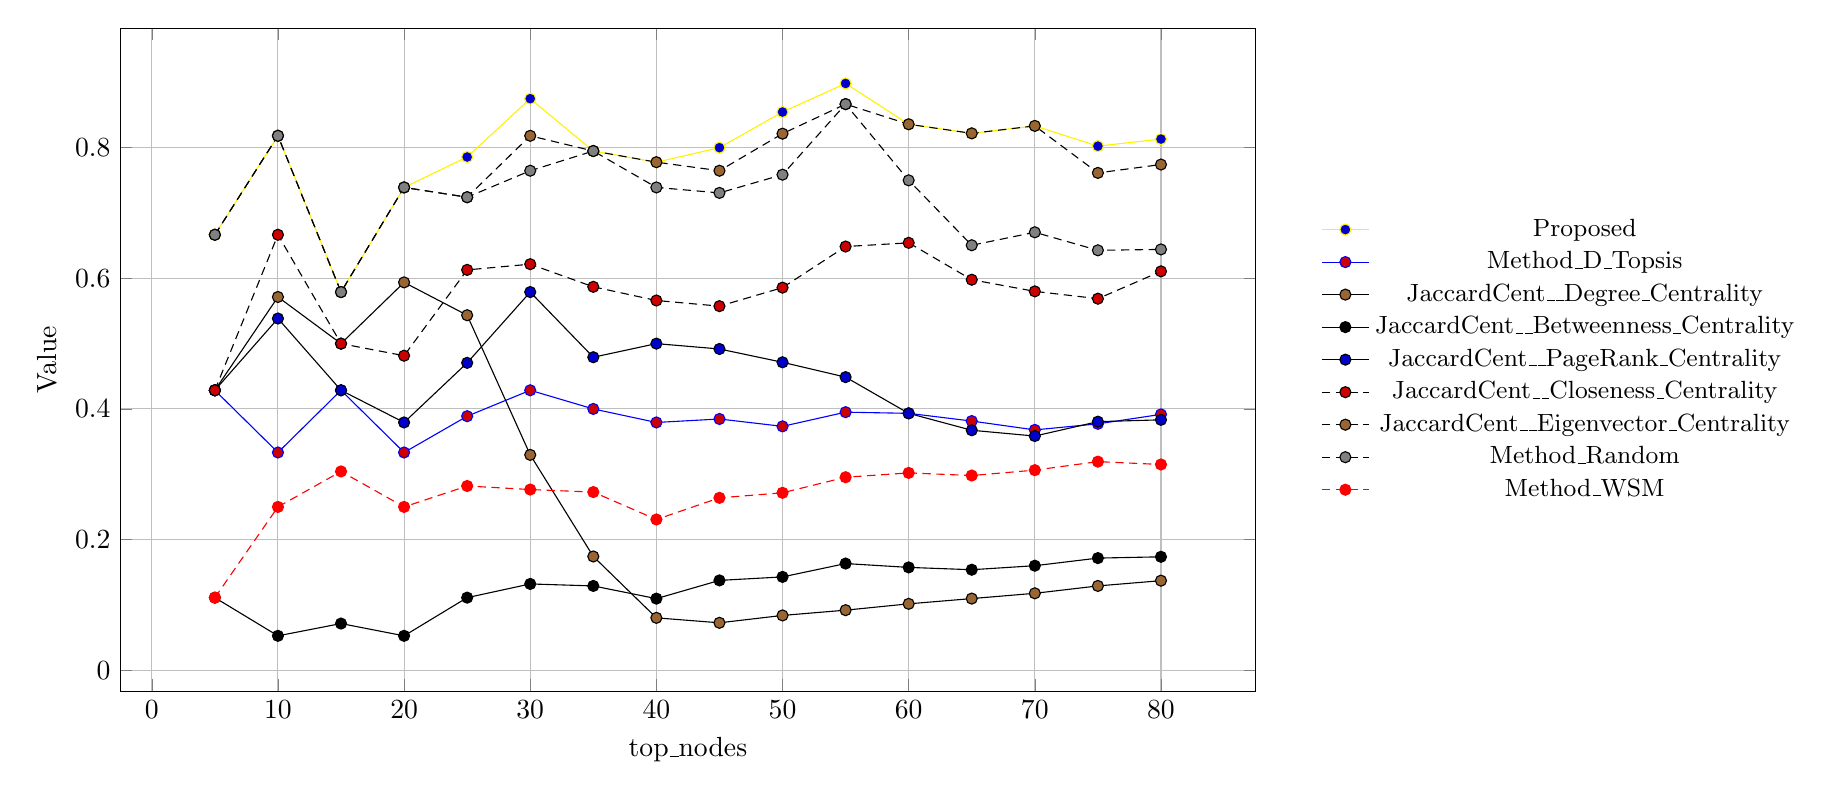
\begin{tikzpicture}
\begin{axis}[
    width=16cm,
    height=10cm,
    xlabel={top\_nodes},
    ylabel={Value},
    grid=major,
    legend style={
        at={(1.05,0.5)},
        anchor=west,
        font=\small,
        draw=none,
        cells={align=left},
    },
]
% Proposed
\addplot+[color=yellow, mark=*] coordinates {
(5.0,0.6666666666666666) (10.0,0.8181818181818182) (15.0,0.5789473684210527) (20.0,0.7391304347826086) (25.0,0.7857142857142857) (30.0,0.875) (35.0,0.7948717948717948) (40.0,0.7777777777777778) (45.0,0.8) (50.0,0.8545454545454545) (55.0,0.8983050847457628) (60.0,0.835820895522388) (65.0,0.821917808219178) (70.0,0.8333333333333334) (75.0,0.8023255813953488) (80.0,0.8131868131868132) };
\addlegendentry{Proposed}

% Method\_D\_Topsis
\addplot+[color=blue, mark=*] coordinates {
(5.0,0.4285714285714285) (10.0,0.3333333333333333) (15.0,0.4285714285714285) (20.0,0.3333333333333333) (25.0,0.3888888888888889) (30.0,0.4285714285714285) (35.0,0.4) (40.0,0.3793103448275862) (45.0,0.3846153846153846) (50.0,0.3733333333333333) (55.0,0.3950617283950617) (60.0,0.3932584269662921) (65.0,0.3814432989690721) (70.0,0.3679245283018867) (75.0,0.3771929824561403) (80.0,0.3916666666666666) };
\addlegendentry{Method\_D\_Topsis}

% JaccardCent\_\_Degree\_Centrality
\addplot+[color=black, mark=*] coordinates {
(5.0,0.4285714285714285) (10.0,0.5714285714285714) (15.0,0.5) (20.0,0.59375) (25.0,0.5434782608695652) (30.0,0.3296703296703296) (35.0,0.1741293532338308) (40.0,0.0801603206412825) (45.0,0.0725806451612903) (50.0,0.0838709677419354) (55.0,0.0919354838709677) (60.0,0.1016129032258064) (65.0,0.1096774193548387) (70.0,0.1177419354838709) (75.0,0.1290322580645161) (80.0,0.1370967741935483) };
\addlegendentry{JaccardCent\_\_Degree\_Centrality}

% JaccardCent\_\_Betweenness\_Centrality
\addplot+[color=black, mark=*] coordinates {
(5.0,0.1111111111111111) (10.0,0.0526315789473684) (15.0,0.0714285714285714) (20.0,0.0526315789473684) (25.0,0.1111111111111111) (30.0,0.1320754716981132) (35.0,0.1290322580645161) (40.0,0.1095890410958904) (45.0,0.1375) (50.0,0.1428571428571428) (55.0,0.1632653061224489) (60.0,0.1574074074074074) (65.0,0.1538461538461538) (70.0,0.16) (75.0,0.1716417910447761) (80.0,0.1736111111111111) };
\addlegendentry{JaccardCent\_\_Betweenness\_Centrality}

% JaccardCent\_\_PageRank\_Centrality
\addplot+[color=black, mark=*] coordinates {
(5.0,0.4285714285714285) (10.0,0.5384615384615384) (15.0,0.4285714285714285) (20.0,0.3793103448275862) (25.0,0.4705882352941176) (30.0,0.5789473684210527) (35.0,0.4791666666666667) (40.0,0.5) (45.0,0.4918032786885246) (50.0,0.4714285714285714) (55.0,0.4487179487179487) (60.0,0.3932584269662921) (65.0,0.3673469387755102) (70.0,0.3584905660377358) (75.0,0.3805309734513274) (80.0,0.3833333333333333) };
\addlegendentry{JaccardCent\_\_PageRank\_Centrality}

% JaccardCent\_\_Closeness\_Centrality
\addplot+[color=black, mark=*] coordinates {
(5.0,0.4285714285714285) (10.0,0.6666666666666666) (15.0,0.5) (20.0,0.4814814814814814) (25.0,0.6129032258064516) (30.0,0.6216216216216216) (35.0,0.5869565217391305) (40.0,0.5660377358490566) (45.0,0.5573770491803278) (50.0,0.5857142857142857) (55.0,0.6486486486486487) (60.0,0.654320987654321) (65.0,0.5978260869565217) (70.0,0.58) (75.0,0.5688073394495413) (80.0,0.6106194690265486) };
\addlegendentry{JaccardCent\_\_Closeness\_Centrality}

% JaccardCent\_\_Eigenvector\_Centrality
\addplot+[color=black, mark=*] coordinates {
(5.0,0.6666666666666666) (10.0,0.8181818181818182) (15.0,0.5789473684210527) (20.0,0.7391304347826086) (25.0,0.7241379310344828) (30.0,0.8181818181818182) (35.0,0.7948717948717948) (40.0,0.7777777777777778) (45.0,0.7647058823529411) (50.0,0.8214285714285714) (55.0,0.8666666666666667) (60.0,0.835820895522388) (65.0,0.821917808219178) (70.0,0.8333333333333334) (75.0,0.7613636363636364) (80.0,0.7741935483870968) };
\addlegendentry{JaccardCent\_\_Eigenvector\_Centrality}

% Method\_Random
\addplot+[color=black, mark=*] coordinates {
(5.0,0.6666666666666666) (10.0,0.8181818181818182) (15.0,0.5789473684210527) (20.0,0.7391304347826086) (25.0,0.7241379310344828) (30.0,0.7647058823529411) (35.0,0.7948717948717948) (40.0,0.7391304347826086) (45.0,0.7307692307692307) (50.0,0.7586206896551724) (55.0,0.8666666666666667) (60.0,0.75) (65.0,0.6506024096385542) (70.0,0.6704545454545454) (75.0,0.6428571428571429) (80.0,0.6442307692307693) };
\addlegendentry{Method\_Random}

% Method\_WSM
\addplot+[color=red, mark=*] coordinates {
(5.0,0.1111111111111111) (10.0,0.25) (15.0,0.3043478260869565) (20.0,0.25) (25.0,0.282051282051282) (30.0,0.2765957446808511) (35.0,0.2727272727272727) (40.0,0.2307692307692307) (45.0,0.2638888888888889) (50.0,0.2716049382716049) (55.0,0.2954545454545454) (60.0,0.3020833333333333) (65.0,0.2980769230769231) (70.0,0.3063063063063063) (75.0,0.3193277310924369) (80.0,0.3149606299212598) };
\addlegendentry{Method\_WSM}


\end{axis}
\end{tikzpicture}

\end{document}
